\documentclass[10pt]{beamer}
\usepackage[space,hyperref,UTF8]{ctex} %ctex中文宏包
\usepackage{gbt7714}
\setbeamertemplate{caption}[numbered] %给表格和图片设置计数器
	
\setbeamertemplate{navigation symbols}{} %取消掉导航符号的显示

\usetheme{warsaw} %beamer主题,beamer因为有各种主题才使得有生气
%常用的:warsaw Antibes Bergen  Berkeley Berlin Boadilla Copenhagen Darmstadt Dresden Frankfurt Goettingen Hannover Ilmenau Juanlespins Madrid Malmoe Marburg Montpellier Paloalto Pittsburgh Rochester Singapore

\usecolortheme{default} %颜色主题

\title[short title]{long long title}
\subtitle[short subtitle]{long subtitle}
\author[short author name]{long author name}
\date[short date]{long date}
\institute[short Ins name]{long ins name}
\titlegraphic{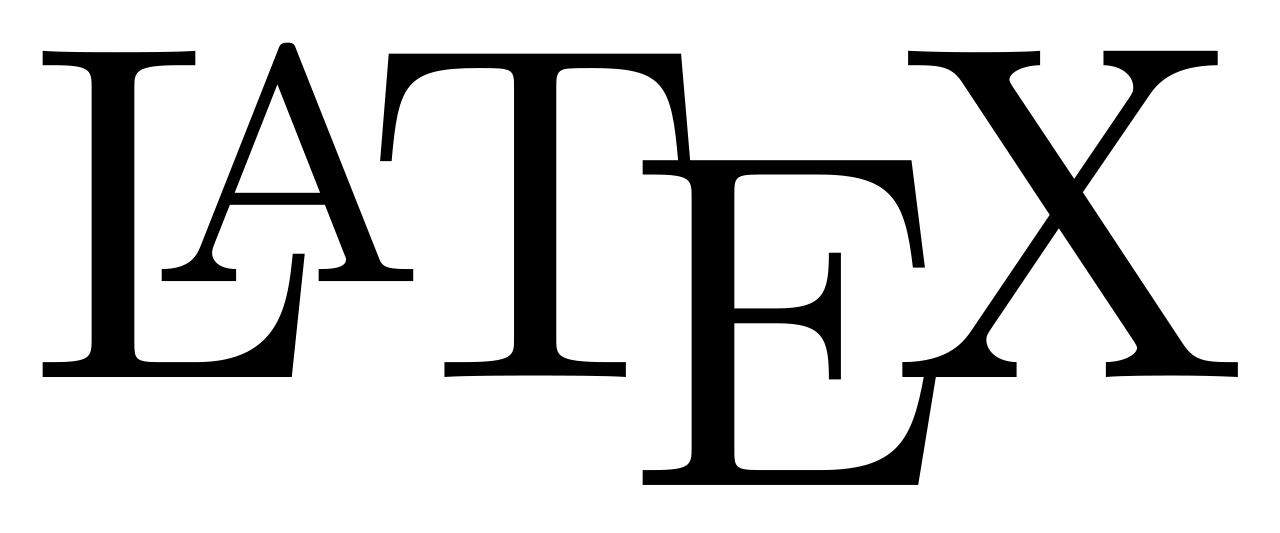
\includegraphics[width=0.5\textwidth]{./logo/LaTex.png}}

\begin{document}
	\frame{\titlepage} %标题帧
	\begin{frame}[c]\frametitle{分栏}
	\begin{columns}  %多栏环境,beamer用columns,LATEX用minipage
		\column{.49\textwidth} %栏宽大概占一半,小于1
		First column text and/or code
		\begin{itemize}		%无序列表itemize示例
			\item The first item
			\item The second item
			\item The third item
			\item The fourth item
		\end{itemize}
		\column{.49\textwidth}
		Second column text and/or code
		\begin{enumerate}	%有序列表enumerate示例
			\item The first item
			\item The second item
			\item The third item
			\item The fourth item
		\end{enumerate}
	\end{columns}
	\end{frame}

	%beamer的特色功能:区块(block)
	\begin{frame}[c]{区块}  %适用于各种定理,引理以及示例
		\begin{theorem}[勾股定理]
			勾三股四弦五\centering
			\begin{equation}
				a^2 + b^2 = c^2
			\end{equation}
		\end{theorem}
		
		\begin{example} %示例环境
			this is the example block environment.
		\end{example}
	
		
%		\begin{lemma} %引理环境
%			this is  the lemma envir.
%		\end{lemma}
	
		\begin{proof}  %证明环境
			this is the proof envir.
		\end{proof}
	
%		\begin{corollary}%推论环境
%			this is the corollary envir.
%		\end{corollary}
	
		\begin{alertblock}{alert}%推论环境
			this is the alertblock envir.
		\end{alertblock}
	
	\end{frame}

	\begin{frame}[c]{beamer插入表格和\LaTeX 没有区别}
		\begin{table}[t] %h表示here, t –top, b-bottom
			\centering
			\caption{表格标题\label{tab:biaoge}}
		\begin{tabular}{|c|c|}
			\hline 
			1 & 2 \\ 
			\hline 
			4 & 3 \\ 
			\hline 
		\end{tabular} 
		\end{table}
	\end{frame}

	\begin{frame}[c]{beamer插入图片和\LaTeX 没有区别}
	\begin{table}[htb!] %h表示here, t –top, b-bottom;[htb]是按照其顺序排列进行选择,即h, t ,b顺序.
		\begin{figure}
			\centering
			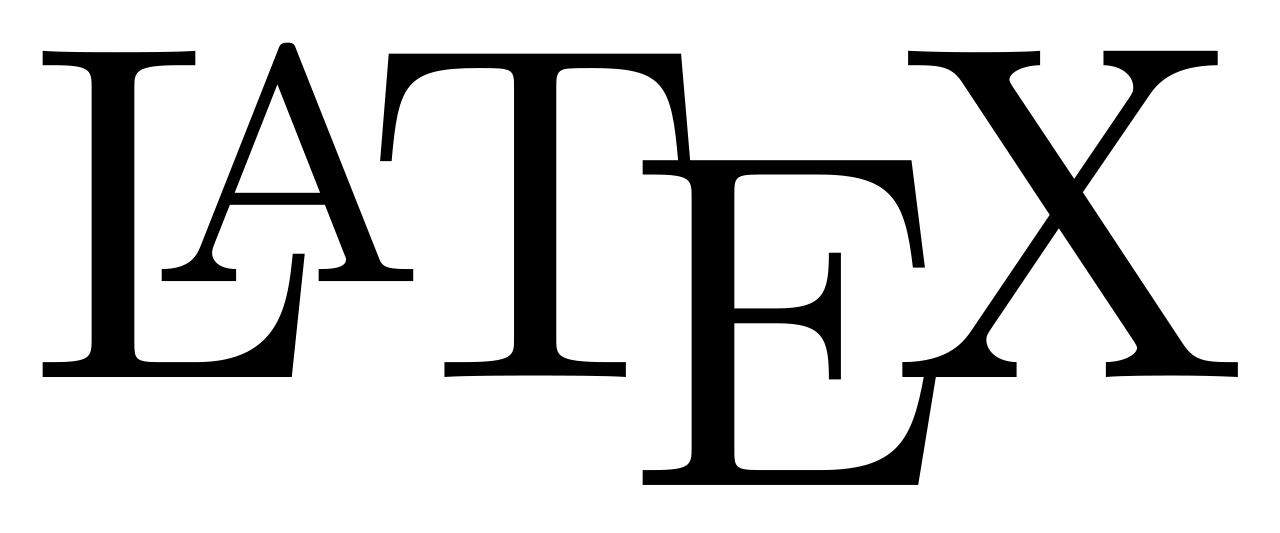
\includegraphics[width=0.9\linewidth]{logo/LaTex}
			\caption{LaTex Picture}
			\label{fig:LaTex}
		\end{figure}
	\end{table}	
	\end{frame}

	\begin{frame}[c]{文献正文引用}
		this is\cite{.2004b} a reference\cite{RN142} envir\cite{.2005b}.
		
		this\cite{.2004d} is the\cite{RN142} another\cite{RN94} reference\cite{.2005c}.
	\end{frame}

	\begin{frame}[t,allowframebreaks]{References} %使用 allowframebreaks 选项是为了自动分帧
	\def\newblock{}
	%\bibliographystyle{unsrt}
	\bibliography{20181115}
	\end{frame}

\end{document}
%website:http://ddswhu.com/beamer-tips/
%website:http://ddswhu.com/beamer-tutoriral/